\documentclass[review]{elsarticle}

\usepackage[colorlinks]{hyperref}
\usepackage[colorinlistoftodos]{todonotes}
\usepackage{verbatim}
\usepackage[utf8]{inputenc}
\usepackage[T1]{fontenc}
\usepackage{adjustbox}
\usepackage{multirow}
\usepackage{longtable}
\usepackage{booktabs}
\usepackage{lineno,hyperref}
\usepackage{float}
\modulolinenumbers[5]

\journal{colleagues for review}

%%%%%%%%%%%%%%%%%%%%%%%
%% Elsevier bibliography styles
%%%%%%%%%%%%%%%%%%%%%%%
%% APA style
\bibliographystyle{model5-names}\biboptions{authoryear}
%%%%%%%%%%%%%%%%%%%%%%%

\begin{document}

\begin{frontmatter}

\title{Shape as a function of time + raw material + burial context: An exploratory analysis of Perdiz arrow point shape from the southern Caddo area}

%% Group authors per affiliation:
\author{Robert Z. Selden, Jr.\textsuperscript{a,b,c}*, John E. Dockall\textsuperscript{d,e}, C. Britt Bousman\textsuperscript{f,g}, and Timothy K. Perttula\textsuperscript{h}}
\address[1]{Heritage Research Center, Stephen F. Austin State University, US}
\address[2]{Cultural Heritage Department, Jean Monnet University, FR}
\address[3]{ORCID ID \href{http://orcid.org/0000-0002-1789-8449}{0000-0002-1789-8449}}
\address[4]{Cox|McClain Environmental Consulting, Inc., US}
\address[5]{ORCID ID \href{http://orcid.org/0000-0002-0940-7144}{0000-0002-0940-7144}}
\address[6]{Department of Anthropology, Texas State University, US}
\address[7]{ORCID ID \href{http://orcid.org/0000-0002-1645-8302}{0000-0002-1645-8302}}
\address[8]{Archeological \& Environmental Consultants, LLC, US}
\cortext[cor1]{Corresponding author, Robert Z. Selden, Jr. (zselden@sfasu.edu)}

\begin{abstract}
Temporal assignments carry substantive weight in archaeological practice, and it is regularly assumed that artefacts from different temporal units may have differed in ways that convey changes in preference or behaviour. Similarly, archaeologists regularly assume that raw material differences articulate with stone tool morphology, and the role of differential raw material quality and preference associated with Caddo lithic technology remains largely unexplored. Whether a particular artefact is found in or outside of burial contexts is a sensitive and regularly discussed topic in the archaeological literature, providing valuable insights related to prehistoric burial practices, as well as generational shifts in aesthetics, design, and raw material preferences. These assumptions were tested using geometric morphometrics, yielding results in support of the hypothesis that Perdiz arrow point shape is protean, and that significant differences existed in shape by time, raw material, and burial context in the southern Caddo area.
\end{abstract}

\begin{keyword}
NAGPRA \sep computational archaeology \sep digital archaeology \sep museum studies \sep digital humanities
\end{keyword}

\end{frontmatter}

\linenumbers

\section*{}

\begin{quote}
The assumption is that the ability to execute formal technological designs is severely limited by the quality of the raw material. Toolkits based on high quality raw materials are thought to be easier to design because fracture is easier to control \citep{RN4315,RN8924}. In contrast, toolkits based on poor quality raw material are more difficult to design because fracture is unpredictable and results in severe, irreparable errors during reduction. Even where low raw material abundance would encourage formal technological design, raw material quality is thought to be the overriding factor constraining lithic technological organization \citep[257]{RN5907}.
\end{quote}

East Texas geologic formations are poor in lithic raw materials \citep[Figure 2.1]{RN439}, or at least knappable lithic raw materials (Figure ~\ref{fig:raw.map}). Consequently, the scarce lithic raw materials suitable for the manufacture of Perdiz arrow points would have been carefully conserved by the sedentary aboriginal Caddo populations of east Texas (CE 900 - 1680+). In the general east Texas area, only the Pisgah Ridge chert in the Trinity River basin, Manning fused glass in the Manning Formation (part of the Jackson group of Eocene age), and various cherts and quartzites in the Catahoula Formation---exposed in the Neches River basin---are in “geological formations that contain in situ rocks suitable for the manufacture of stone tools” \citep[49]{RN439}. Upland stream gravels are relatively widespread throughout parts of east Texas \citep[56-57]{RN439}. High quality and knappable cobbles of chert, novaculite, and quartzite are present in the Red River gravels in northeastern Texas (also the Bowie gravels of the Red-Sulphur River interfluve, per \citet{RN846}), which derive from chert-bearing formations in the Ouachita Mountains of southeastern Oklahoma (Figure ~\ref{fig:raw.map}) \citep[Figure 1.20]{RN439}.

\begin{figure}[!]\centering
\includegraphics[width=0.95\linewidth]{raw.mat.map.jpg}
\caption{Map of east Texas counties, and potential raw material source areas.}
\label{fig:raw.map}
\end{figure}

According to a study of lithic raw material sources in the Neches River basin by \citet[69]{RN1253}, there are redeposited gravels on stream terraces that contain small cobbles and pebbles of silicified wood, fine-grained quartzite, and various cherts. Local cherts tend to be red, gray, tan, and brown in color \cite[66]{RN1253}. Non-local cherts found at sites in the Neches and Angelina river basins are apparently from central Texas Edwards Plateau sources, and are lustrous gray, blue-gray, and dark brown in colour \citep{RN1253}.

Local lithic raw materials include coarse- and fine-grained quartzite, silicifed wood, ferruginous sandstone, jasper, and several varieties of earth-toned cherts that are yellowish-brown, gray, red, light brown, brown, greenish-brown, and reddish-brown in colour. Non-local raw materials are white and red novaculite, black chert, dark gray chert, white chert, bluish-gray chert, a yellowish-red chert, and quartz. A distinctive coarse-grained quartzite (or metaquartzite) may occur in this general area, although it may be restricted to localised sources. The material is described by \citet[67]{RN1253} as being of sugary coarse-grained texture and light gray to yellowish-brown in colour, and may originate in the Glover Sandstone (part of the basal Sparta Sand Formation) in northeastern Houston County (Figure ~\ref{fig:raw.map}) \cite[69]{RN1253}. A quarry of grayish-white quartzite is known in the Sabine River basin in Van Zandt County (41VN39), which has been noted to turn pink when heat-treated \citep{RN1898}.

The most likely contributing source(s) of non-local cherts used in the manufacture of Perdiz arrow points in northeast and east Texas are those from various Edwards Formation localities in central Texas \citep{RN439,RN2145}. These resources occur in a region that encompasses the Edwards Plateau and the southern Llano Estacado as both massive ledge and cobble varieties. Raw materials also occur as significant gravel sources along the Colorado and Brazos River valleys, and reworked or lagged members of Uvalde Gravel deposits.

\subsection*{Shape, raw material, and human behaviour}

Perdiz arrow points (\citealp[283 and Plate 142]{RN7795}; \citealp[504 and Plate 131]{RN5769}) include a broad distribution across most of Texas from the Rio Grande eastward to the Neches and Angelina River basins, and from the Red River (Texas and Oklahoma) south to the eastern and central parts of the Gulf Coast, and have been noted to include more variation in both size and proportion than most arrow point types found in Texas. In outline, Perdiz arrow points have a “[t]riangular blade with edges usually quite straight but sometimes slightly convex or concave. Shoulders sometimes at right angles to stem but usually well barbed. Stem contracted, often quite sharp at base, but may be somewhat rounded. Occasionally, specimen may be worked on one face only or mainly on one face…[w]orkmanship generally good, sometimes exceedingly fine with minutely serrated blade edges” \cite[504]{RN5769}. 

Perdiz arrow points fall within what \citet[738-741]{RN5873} referred to as a reliable tool; however, unlike dart points, the morphological attributes of arrow points---generally small and thin---somewhat limit discussions of optimisation related to planned breakage caused by impact \citep{RN6170,RN7045}, providing for differing expressions of maintainability \citep{RN5789}. The anticipated exploitation of raw material resources, coupled with the perceived technological advantages of using heat treatment \citep{RN6171}, may have resulted in longer and larger flakes (and more of them), provided the stone reached the requisite temperature \citep{RN5900}. Thermal properties of locally-available raw materials remain ill-understood in the southern Caddo area, and it is unclear whether Caddo knappers enlisted expedient \citep{RN8970,RN6201}, slow and steady \citep{RN8971}, or hybrid approaches to heat treatment.

Inferences regarding human behaviour drawn from stone tool raw material source use patterns are predicated on accurate knowledge of the location of those sources actually used \citep[365]{RN5787}. Similarly, reduction models rooted in knapping experiments make an assumption that the reduction process is known \citep{RN6855}; however, experiments have illustrated that numerous manufacturing strategies could be employed to generate the same products \citep{RN8968,RN8969}. 

\section*{Perdiz arrow point sample}

The sample of whole/intact Perdiz arrow points used for this analysis comes from Anderson, Camp, Harrison, Houston, Nacogdoches, San Augustine, Smith, and Shelby counties (\href{https://aksel-blaise.github.io/perdiz/spatial.html}{supplementary materials} and \citealt{RN8980}), consists of 142 whole/intact Perdiz arrow points from 20 sites across the southern Caddo area, and were manufactured using chert, quartzite, and silicified wood (Figure ~\ref{fig:raw.mat}a). Raw material distributions differ among sites, and chert was preferred across the largest geography (Figure ~\ref{fig:raw.mat}a). Use of quartzite was limited to Camp, Harrison, and Houston counties (Figure ~\ref{fig:raw.mat}a), silicified wood was employed for Perdiz manufacture in Houston, Nacogdoches, and Shelby counties; however, Washington Square Mound (41NA49) is the only burial context where silicified wood Perdiz points have been recovered (Figure ~\ref{fig:raw.mat}a).

All three raw material types are present in Caddo burials, (Figure ~\ref{fig:raw.mat}b); however, raw materials differ through the Middle, Late, and Historic Caddo periods, where chert, quartzite, and silicified wood are present throughout all three periods, but quartzite only occurs in Middle and Late Caddo contexts (Figure ~\ref{fig:raw.mat}c). Radiocarbon and relative dates are discussed in more detail below, and the median of the temporal range was used to assign the Perdiz points to the appropriate temporal period (Middle Caddo, CE 1250-1450; Late Caddo, CE 1450-1680; and Historic Caddo, CE 1680+) (Figure ~\ref{fig:raw.mat}d).

\begin{figure}[!]\centering
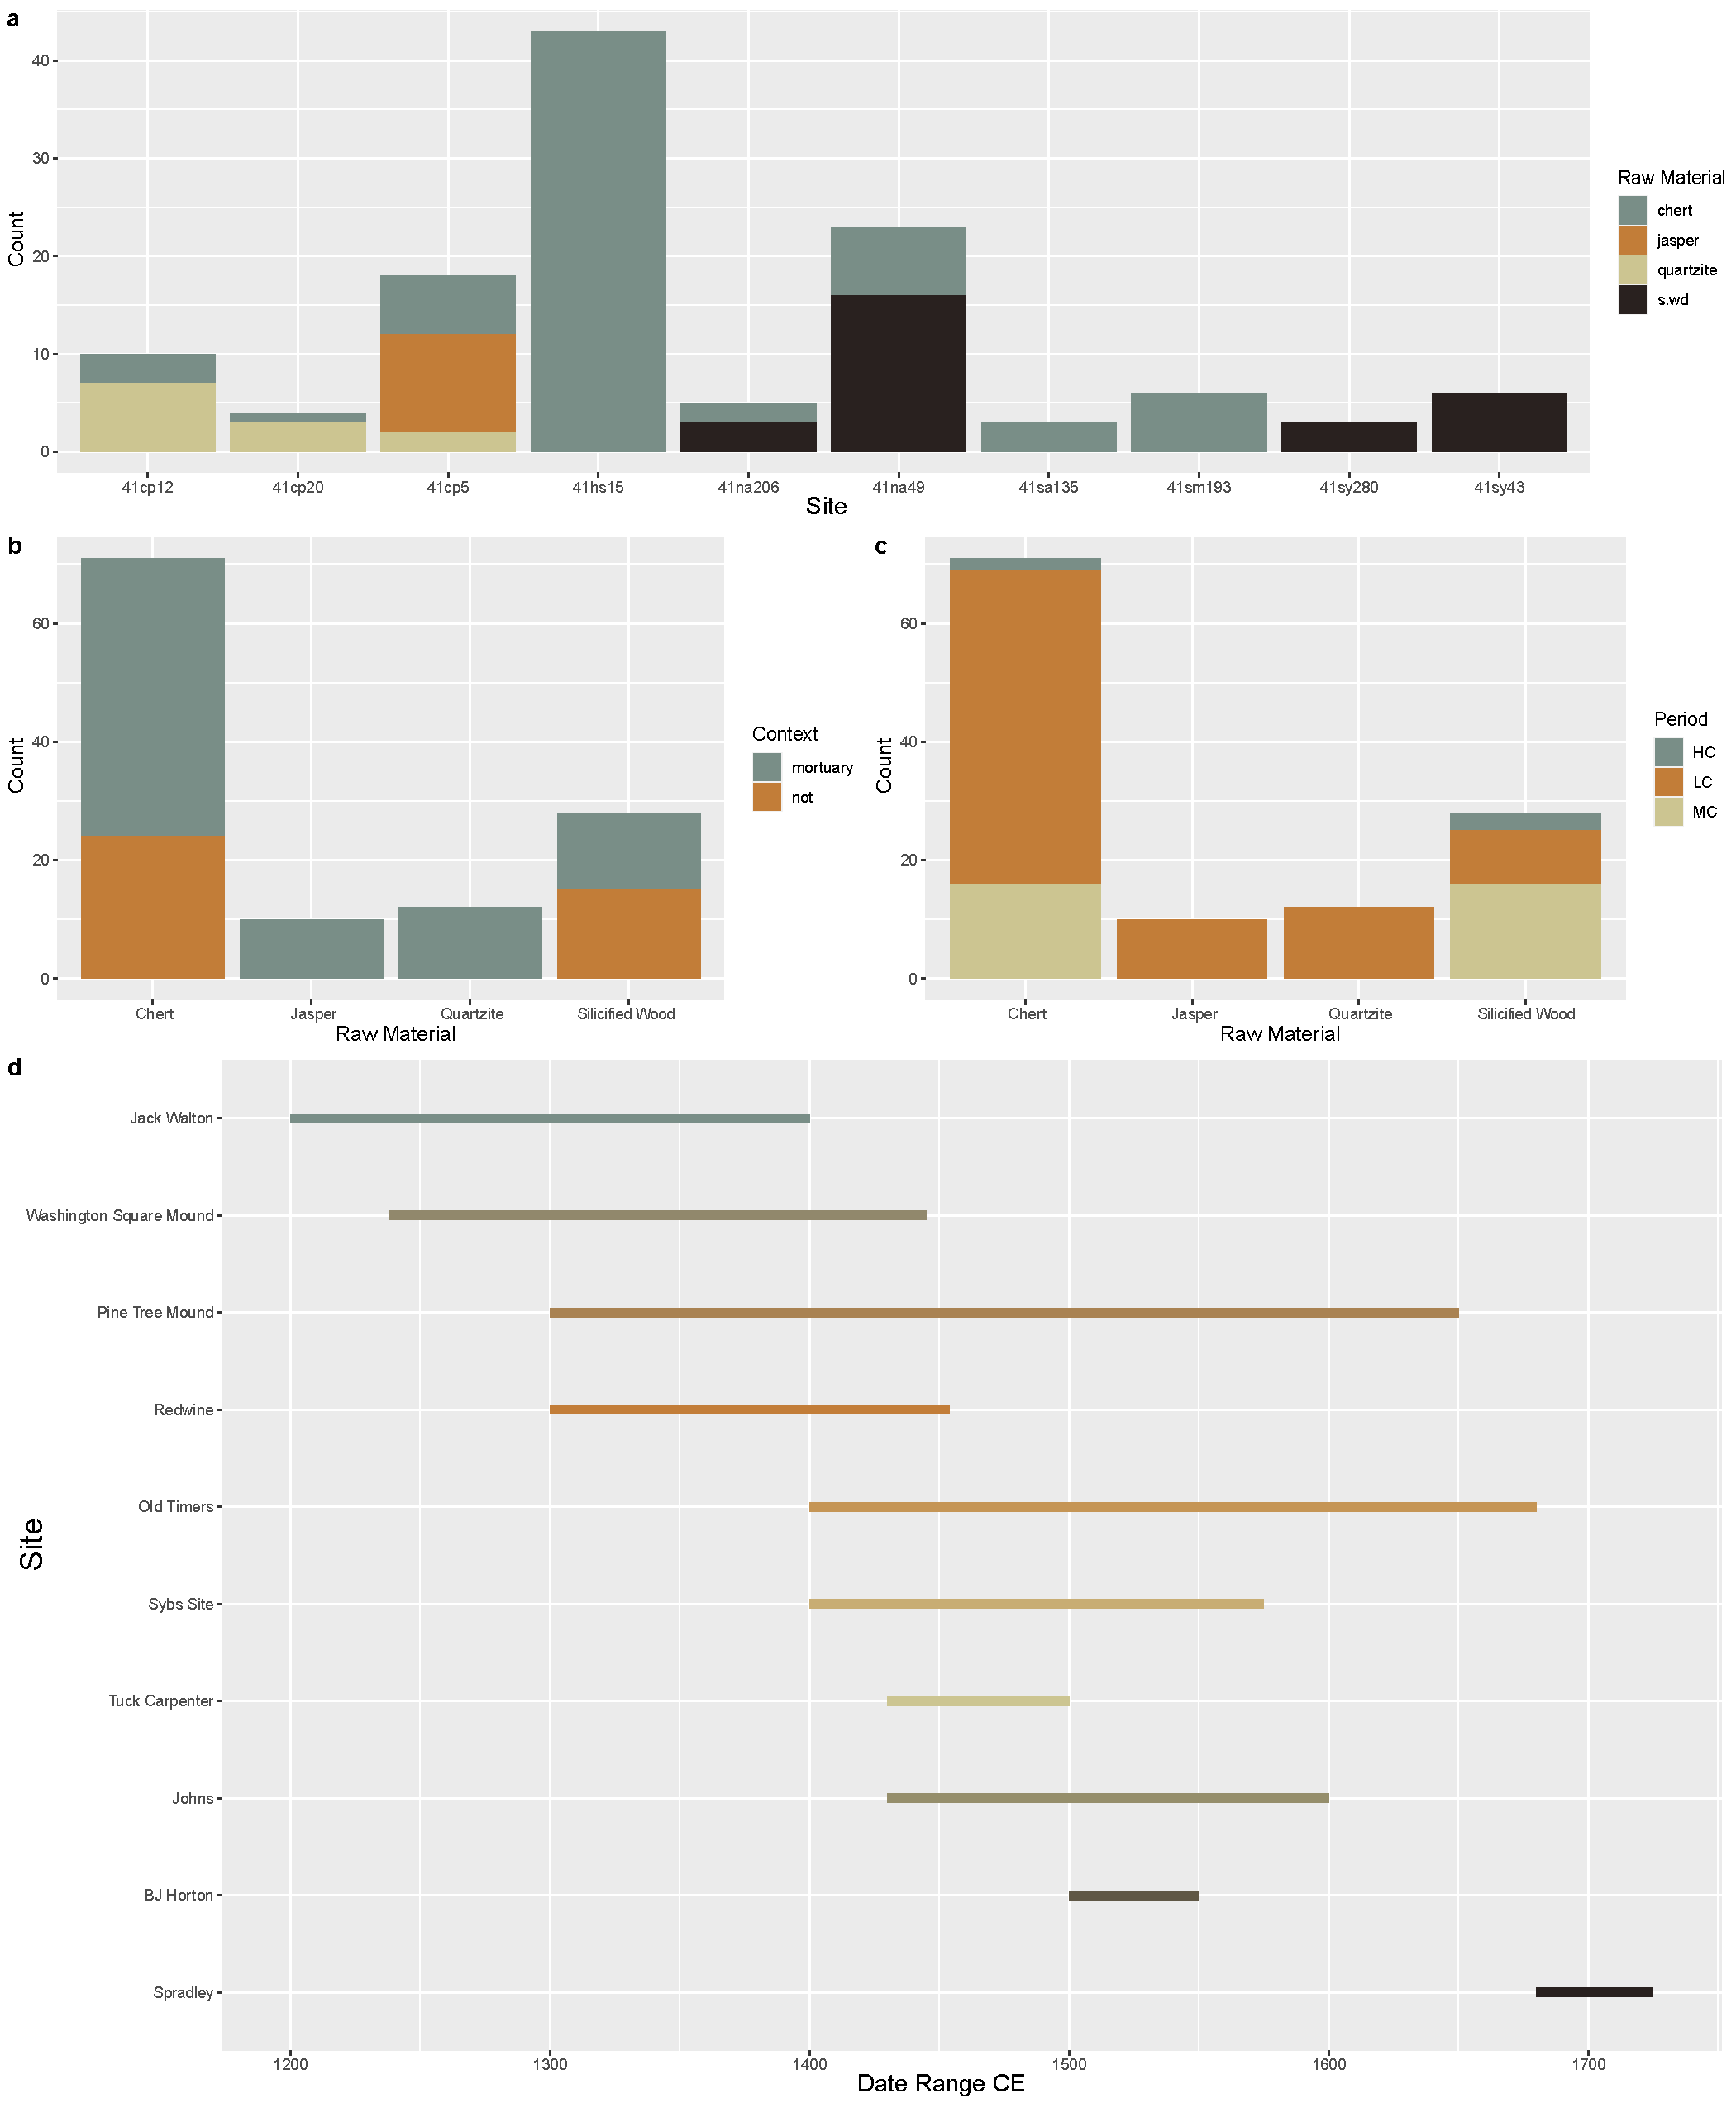
\includegraphics[width=\linewidth]{fig.mat.temp.pdf}
\caption{Raw materials a, by site; b, by mortuary context; c, by temporal period (Middle, Late, or Historic Caddo), and d, temporal range of contexts by site in the Perdiz sample. Additional information related to this figure, including the full results and code needed to reproduce it, can be found in the supplemental materials at \href{https://aksel-blaise.github.io/perdiz/raw-material.html}{https://aksel-blaise.github.io/perdiz/raw-material.html} \citep{RN8980}.}
\label{fig:raw.mat}
\end{figure}

\subsection*{41AN51, Pace McDonald}

The Pace McDonald site (41AN51) is a prehistoric Caddo mound center and associated settlement in the upper Neches River basin of east Texas that was established and occupied during the Middle Caddo period (CE 1250-1450). Nine Perdiz arrow points from habitation contexts are in the collections from the site, including eight made from non-local chert (primarily Edwards Plateau chert from Central Texas) and one from a local chert \citep{RN2444}.

\subsection*{41AN115}

This multi-component prehistoric site is on Town Creek in the Trinity River basin \citep{RN8982}. Diagnostic projectile points recovered at the site suggest it was occupied from Late Paleoindian times to the Woodland period. There is also a small post-CE 900 ancestral Caddo component marked by three grog-tempered ceramic sherds and one Perdiz point from occupational deposits. The Perdiz point is made from a non-local black chert.

\subsection*{41CP5, Tuck Carpenter}

The Tuck Carpenter site is a well-studied Late Caddo period Titus phase cemetery on Dry Creek in the Big Cypress Creek basin, and was used by the Caddo from the 15th to the 17th century. Burials with Perdiz points are the earliest in the cemetery, and likely date from CE 1450-1500 \citep[197]{RN8962}. A single radiocarbon date was obtained from Burial 10: 360 $\pm$ 60 BP. The calibrated age range at 2 sigma is CE 1442-1646, with a median probability of CE 1546 (supplementary materials, and \citealp{RN8980}).

Fifty seven Perdiz points have been recovered from burial features at the Tuck Carpenter site \citep{RN8963,RN3158,RN3159}. A second collection from the site includes an additional 18 Perdiz points from 13 burial features manufactured using Ogallala quartzite and local chert gravel sources; including one that was made from a non-local novaculite \citep[Table 2]{RN8962}.

\subsection*{41CP12, Johns}

The Johns site is a Titus phase cemetery in the Prairie Creek valley of the Big Cypress Creek basin. No radiocarbon dates were obtained from the site, but the decorative motifs associated with the ceramic vessels recovered from burials suggest that the cemetery was used from CE 1450-1600 \citep{RN2440}. Forty-eight Perdiz points were recovered from 16 burial features. They were made from local chert, quartzite, and silicified wood gravel sources (87 percent), non-local sources (10.8 percent, mainly from Red River gravels), and chalcedony (2.2 percent).

\subsection*{41CP20, B. J. Horton}

This ancestral Caddo cemetery in the Big Cypress Creek basin includes at least 19 burials, from which two Perdiz points were recovered \citep[9]{RN2439}. Use of the cemetery by the Caddo occurred primarily between CE 1500-1550 \citep[494]{RN8964}.

\subsection*{41CP220, Kitchen Branch}

The Kitchen Branch site is located on a small tributary to Prairie Creek in the Big Cypress Creek basin. It is a small Titus phase domestic farmstead occupied during the 15th century CE. During archaeological investigations, five Perdiz points were recovered from habitation contexts \citep{RN8964}, which were manufactured from non-local cherts and novaculite \citep[410]{RN8964} likely from Red River gravels.

\subsection*{41CP495, Sam D. Carpenter Bottom}

The Sam D. Carpenter Bottom site rests within an alluvial fan in the Big Cypress Creek valley. It is a single component Late Caddo period Titus phase occupation, likely dating between CE 1500-1550 \citep{RN2275}. Six Perdiz arrow points are in the site collection from habitation contexts, made from local quartzite (16.7 percent), local brown chert (33.3 percent), and non-local cherts (50 percent). The non-local cherts are from the Ouachita Mountains, and include a gray chert and a brownish-black Big Fork chert.

\subsection*{41HS15, Pine Tree Mound Site}

The Pine Tree Mound site is a large Titus phase mound center with associated habitation deposits, family cemeteries, and a large community cemetery \citep{RN5724}. Perdiz arrow points (n = 68) represent 53 percent of the arrow points that could be typed from the site, most (n = 50) from burial contexts and the remainder from habitation deposits. Perdiz points from burial contexts tend to have been made from non-local lithic raw materials, typically chert (42 percent), while none of the non-mortuary Perdiz points are made on non-local raw material \citep[566]{RN5724}.

There are 92 radiocarbon dates available from the Pine Tree Mound site  (\citealp[Table 4.13]{RN5724}; \citealp[Table 2]{RN2944}). Most of the calibrated dates fall between CE 1451-1495 and CE 1397-1429 \citep[Table 3]{RN2944}, but calibrated age ranges suggest that the settlement “was established in the A.D. 1300s and persisted until at least the mid 1600s” \citep[299]{RN5724}.

\subsection*{41HS235, Keasler}

The Keasler site is a Late Caddo Titus phase cemetery on a tributary to Little Cypress Creek \citep{RN8983}. The associated grave goods suggest the cemetery was used by Caddo peoples between CE 1500-1680. The funerary collection from the site includes one Perdiz arrow point made from a local quartzite.

\subsection*{41HS269, C. D. Marsh}

This ancestral Caddo site is on Eight Mile Creek, a southward-flowing tributary of the Sabine River. Habitation deposits here date from CE 1250-1450 \citep{RN1536}, and a single Perdiz point has been recovered from these deposits. This point is made from a non-local grayish-brown chert.

\subsection*{Hickory Creek \#2, Houston County, Texas}

The Hickory Creek \#2 site is on an alluvial rise of Hickory Creek, an eastward-flowing tributary of the Neches River \citep{RN2347}. The site was investigated by the U.S. Forest Service, and has 15th century (Middle Caddo) ancestral Caddo habitation deposits as well as Woodland period deposits. In these deposits are 14 Perdiz arrow points. They are made from local chert (21.4 percent), silicified wood (35.7 percent), local quartzite (35.7 percent), and Glover quartzite (7.1 percent), a non-local raw material that is from the southern Ouachita Mountains and in Red River gravels.

\subsection*{41NA49, Washington Square Mound}

The Washington Square Mound site is located in the Angelina River basin and is a mound center with associated habitation deposits and a cemetery. Excavations in one mound uncovered two shaft tombs with abundant grave goods, but no Perdiz offerings \citep{RN914,RN12}. However, 14 Perdiz points were recovered from a burial feature in the Oak Grove Cemetery portion of the Washington Square Mound site \citep[Figure 77]{RN12}. Another seven Perdiz points came from habitation areas near the main burial mound \citep[Table 14]{RN8963}. Of those, 71 percent are on gray chert of likely central Texas origin, and the remainder were made from local quartzite.

Twelve radiocarbon dates have been obtained from the Washington Square Mound site (\citealp[Table 4]{RN914}; \citealp{RN2944}), indicating use of the site in both Early (CE 900-1250) and Middle Caddo periods (CE 1250-1450). The best dates that can be associated with Perdiz points at the site range from cal. CE 1238-1445.

\subsection*{41NA206, Spradley}

The Spradley site includes late 17th to early 18th century archaeological deposits with European trade goods from habitation deposits in the Bayou La Nana valley in the Angelina River basin \citep{RN8965}. Those habitation deposits, which have no associated radiocarbon dates, contain numerous Perdiz points (n = 31). Approximately 94 percent were manufactured from local silicified wood, quartzite, and gravel cherts, and the remainder are from non-local brownish-gray to translucent gray chert, likely from central Texas raw material sources \citep[Table 7]{RN8965}.

\subsection*{41SA135, Jack Walton}

This site is located on Attoyac Bayou \citep{RN1971}, and is an ancestral Caddo site with habitation deposits of likely Middle Caddo period age (CE 1250-1450). There are no radiocarbon dates from the site. Excavations at the site recovered seven Perdiz points.

\subsection*{41SM55, Bryan Hardy}

The Bryan Hardy site is an ancestral Caddo mound center and settlement on a northern-flowing tributary to the Sabine River \citep{RN3231}. Radiocarbon dates from the site indicate that it dates to the Middle Caddo period, between CE 1297-1391. One serrated Perdiz arrow point was found in habitation deposits (House 3) at the site. It was manufactured from a non-local grayish-white chert.

\subsection*{41SM193, Redwine}

The Redwine site (41SM193) site is a Middle Caddo period component located 22 km from the river on a north-flowing tributary (Auburn Creek) of the Sabine River \citep{RN3230}, which includes habitation deposits and a small cemetery. The site has one calibrated date of CE 1300-1454, at 2 sigma, with a median calibrated probability of CE 1356. The 11 Perdiz points from habitation deposits were manufactured on black, brown, and grayish-tan chert as well as Ogallala quartzite \citep[14]{RN3230}. An additional 13 Perdiz arrow points were among the grave goods recovered from two burial features \citep[35]{RN3230}.

\subsection*{41SM195, Wolf}

The Wolf site is an ancestral Caddo site also on Auburn Creek. A single 2 sigma calibrated radiocarbon date from a feature in habitation deposits ranges from CE 1315-1440 \citep{RN3220}. Two Perdiz arrow points have been recovered from the site, both made of a local brown chert \citep[4,5,Figure 8]{RN3220}.

\subsection*{41SM442, Alligator Pond}

The Alligator Pond site is a multi-component prehistoric habitation site in the Saline Creek valley of the Sabine River basin \citep{RN2375,RN2374}. The principal component by ancestral Caddo peoples is between CE 1000-1300. The lithic tool assemblage includes three Perdiz arrow points of non-local chert \citep[Figure 19c, e, j]{RN2374}.

\subsection*{41SY43, Old Timers'}

The Old Timers site is located in the Sabine River basin, and includes post-CE 1400 Late Caddo habitation deposits concentrated in the northern area of the site. Excavations recovered eight Perdiz points, all with serrated blades and made from cherts, 75 percent local gravel cherts, and an additional 25 percent of gray cherts from non-local raw material sources \citep[77]{RN8966}.

\subsection*{41SY280, Syb’s Site} 

This ancestral Caddo site of the Late Caddo Salt Lick phase is located along the Toledo Bend Reservoir, west of the now inundated Sabine River floodplain \citep[Figure 55]{RN8966}. It has a number of habitation clusters that include daub and fired clay from areas of burned ancestral Caddo house structures. There are no radiocarbon dates from the site, but the decorated ceramic vessel sherds in the collection areas suggest that the site relatively dates to a period beginning at CE 1450 through the late CE 1500s. One Perdiz arrow point was recovered from Area 13 of the site \citep[Table 33]{RN8966}.

\section*{Methods and results}

\subsection*{Chi-square}

Contingency table analyses of Perdiz arrow points were conducted for raw material and burial context for Middle Caddo, and Late and Historic Caddo period sites are presented below. Chi-square, p values, and Cramer’s V were generated using the Real Statistics Resource Pack software add-in for Excel (Charles Zaiontz. \href{www.real-statistics.com}{www.real-statistics.com}. Release 7.2; Copyright 2013 – 2020). Adjusted residuals were calculated following \citet{RN8987}, and are significant at a 0.05 level of confidence if greater or equal to 1.96 or less than or equal to -1.96. 

In the Middle Caddo period, Perdiz points manufactured using silicified wood were found in mortuary contexts while those made using chert, quartzite, and silicified wood were found in non-mortuary contexts (Table ~\ref{tab:Tbl1}). A chi-square test of independence shows that this pattern is significant, and the Cramer’s V Correlation of 0.755 indicates a moderately strong correlation. Adjusted Residuals indicate that chert and silicified wood are both inversely patterned and the main source of variation (Table ~\ref{tab:Tbl2}). Quartzite follows the chert pattern, but does not deviate enough from the expected pattern to be considered significant.

\begin{table}[tbh]\centering
\footnotesize
\caption{Contingency Table for Middle Caddo Perdiz points.}
\centering
\begin{tabular}{lccc}
\hline
 & Mortuary (O/E) & Non-Mortuary (O/E) & Total\\
\hline
Chert & 0/6.9 & 26/19.1 & 26\\
Quartzite & 0/1.1 & 4/3.0 & 4\\
Silicified Wood & 13/5.0 & 1/14.0 & 19\\
\hline
\textbf{Total} & \textbf{13} & \textbf{36} & \textbf{49}\\
\hline
\end{tabular}\\
\textit{$X^{2}$ = 27.94, df = 2, p value = 8.57^{-7}, Cramer’s V = 0.755}
\label{tab:Tbl1}
\end{table}

\begin{table}[tbh]\centering
\footnotesize
\caption{Adjusted residuals for Middle Caddo Perdiz points; adjusted residuals are significant at a 0.05 level of confidence if \textbf{\geq 1.96} or \textbf{\leq -1.96}.}
\centering
\begin{tabular}{lcc}
\hline
 & Mortuary & Non-Mortuary\\
\hline
Chert & \textbf{-4.47} & \textbf{4.47}\\
Quartzite & -1.26 & 1.24\\
Silicified Wood & \textbf{5.28} & \textbf{-5.29}\\
\hline
\end{tabular}\\
\textit{CV\alpha 0.05 \geq1.96 or \leq-1.96}
\label{tab:Tbl2}
\end{table}

The contingency table analysis for Late and Historic Caddo periods was undertaken using the same methodology and software. The Late and Historic Caddo pattern is the inverse of the Middle Caddo pattern (Table ~\ref{tab:Tbl3}). In the later time periods, only chert and quartzite Perdiz points are found in mortuary contexts, not silicified wood. In non-mortuary contexts, only chert and silicified wood Perdiz points were found. The chi-square shows that the results are significant, and the Cramer’s V correlation indicates the correlation is weaker than in the Middle Caddo comparison above, but still significant. The adjusted residuals indicate that all cells vary significantly from the expected values (Table ~\ref{tab:Tbl4}).

\begin{table}[tbh]\centering
\footnotesize
\caption{Contingency table for Late and Historic Caddo Perdiz points.}
\centering
\begin{tabular}{lccc}
\hline
 & Mortuary (O/E) & Non-Mortuary (O/E) & Total\\
\hline
Chert & 57/51.2 & 11/16.8 & 68\\
Quartzite & 13/9.8 & 0/3.2 & 13\\
Silicified Wood & 0/9.0 & 12/3.0 & 12\\
\hline
\textbf{Total} & \textbf{70} & \textbf{23} & \textbf{93}\\
\hline
\end{tabular}
\label{tab:Tbl3}
\end{table}

\begin{table}[tbh]\centering
\footnotesize
\caption{Adjusted residuals for Late and Historic Caddo Perdiz points; adjusted residuals are significant at a 0.05 level of confidence if \textbf{\geq 1.96} or \textbf{\leq -1.96}.}
\centering
\begin{tabular}{lcc}
\hline
 & Mortuary & Non-Mortuary\\
\hline
Chert & \textbf{3.15} & \textbf{-3.15}\\
Quartzite & \textbf{2.23} & \textbf{-2.23}\\
Silicified Wood & \textbf{-6.48} & \textbf{6.48}\\
\hline
\end{tabular}\\
\textit{CV\alpha 0.05 \geq1.96 or \leq-1.96}
\label{tab:Tbl4}
\end{table}

\subsection*{Elliptical Fourier Analysis}

Two-dimensional (2D) images of the Perdiz arrow points from the Turner collection were collected at a 600dpi resolution as uncompressed tiff files, and all other images were digitised from figures used in articles and technical reports available through the \href{https://scholarworks.sfasu.edu/ita/}{\textit{Index of Texas Archaeology}}. Images were masked in Adobe Photoshop 2021 (v. 22.1.0), exported as jpegs, then imported to R \citep{RN8584}, where the Momocs package was used for an elliptical Fourier analysis (EFA) \citep{RN8925}. EFA is a common tool used for the analysis of stone tool shape \citep{RN2805,RN9003,RN6313,RN5230,RN5225,RN5227,RN8358,RN8967,RN5231,RN7164,RN9004}, and provides visualisations complementary to traditional descriptions, as well as linear and/or orthogonal metrics. The outline of each projectile was retained, and all specimens were normalised to a common centroid, then rescaled using centroid size \citep{RN8923}. 

The \textit{calibrate harmonic power function} was used to identify the number of harmonics necessary to capture Perdiz point shape \citep{RN8925}, and 11 harmonics were retained to achieve 99 percent harmonic power. An exploratory measure (EFA-PCA) was employed to assess variability among time, raw material, and burial context (supplemental materials, \citealt[Chapter 4]{RN8980}). The shape differences among PC1 occur in blade width, while those for PC2 articulate with stem length (supplemental materials, \citealt[Chapter 4]{RN8980}).

\subsubsection*{Shape as a function of time}

Results of the multivariate analysis of variance (MANOVA) through a Hotelling-Lawley of 99 percent cumulative shape variance indicated a significant difference in Perdiz arrow point shape by time (\textit{Hotelling-Lawley}: 1.8209, \textit{F}: 6.1202, \textit{PR(>F)}: 2.23-16) (Figure ~\ref{fig:gmtemp} [top] and supplemental materials, \citealt[Chapter 4]{RN8980}). A subsequent MANOVA with pairwise comparison demonstrated a significant difference in mean Perdiz arrow point shape between each of the three temporal periods (Table ~\ref{tab:tab.shape.time} and supplemental materials, \citealt[Chapter 4]{RN8980}). Mean shapes plotted by temporal periods (Middle, Late, and Historic Caddo) indicate a change in Perdiz arrow point shoulder angles through time, ranging from obtuse in the Middle Caddo period, to acute in the Historic Caddo period (Figure ~\ref{fig:gmtemp}, bottom). This suggests that a shoulder angle-based metric similar to what \citet{RN8275} developed for her analysis of Gary dart points at the Scott site (34Lf-11) may hold added value for temporally-based research questions related to Perdiz arrow points.

\begin{figure}[!]\centering
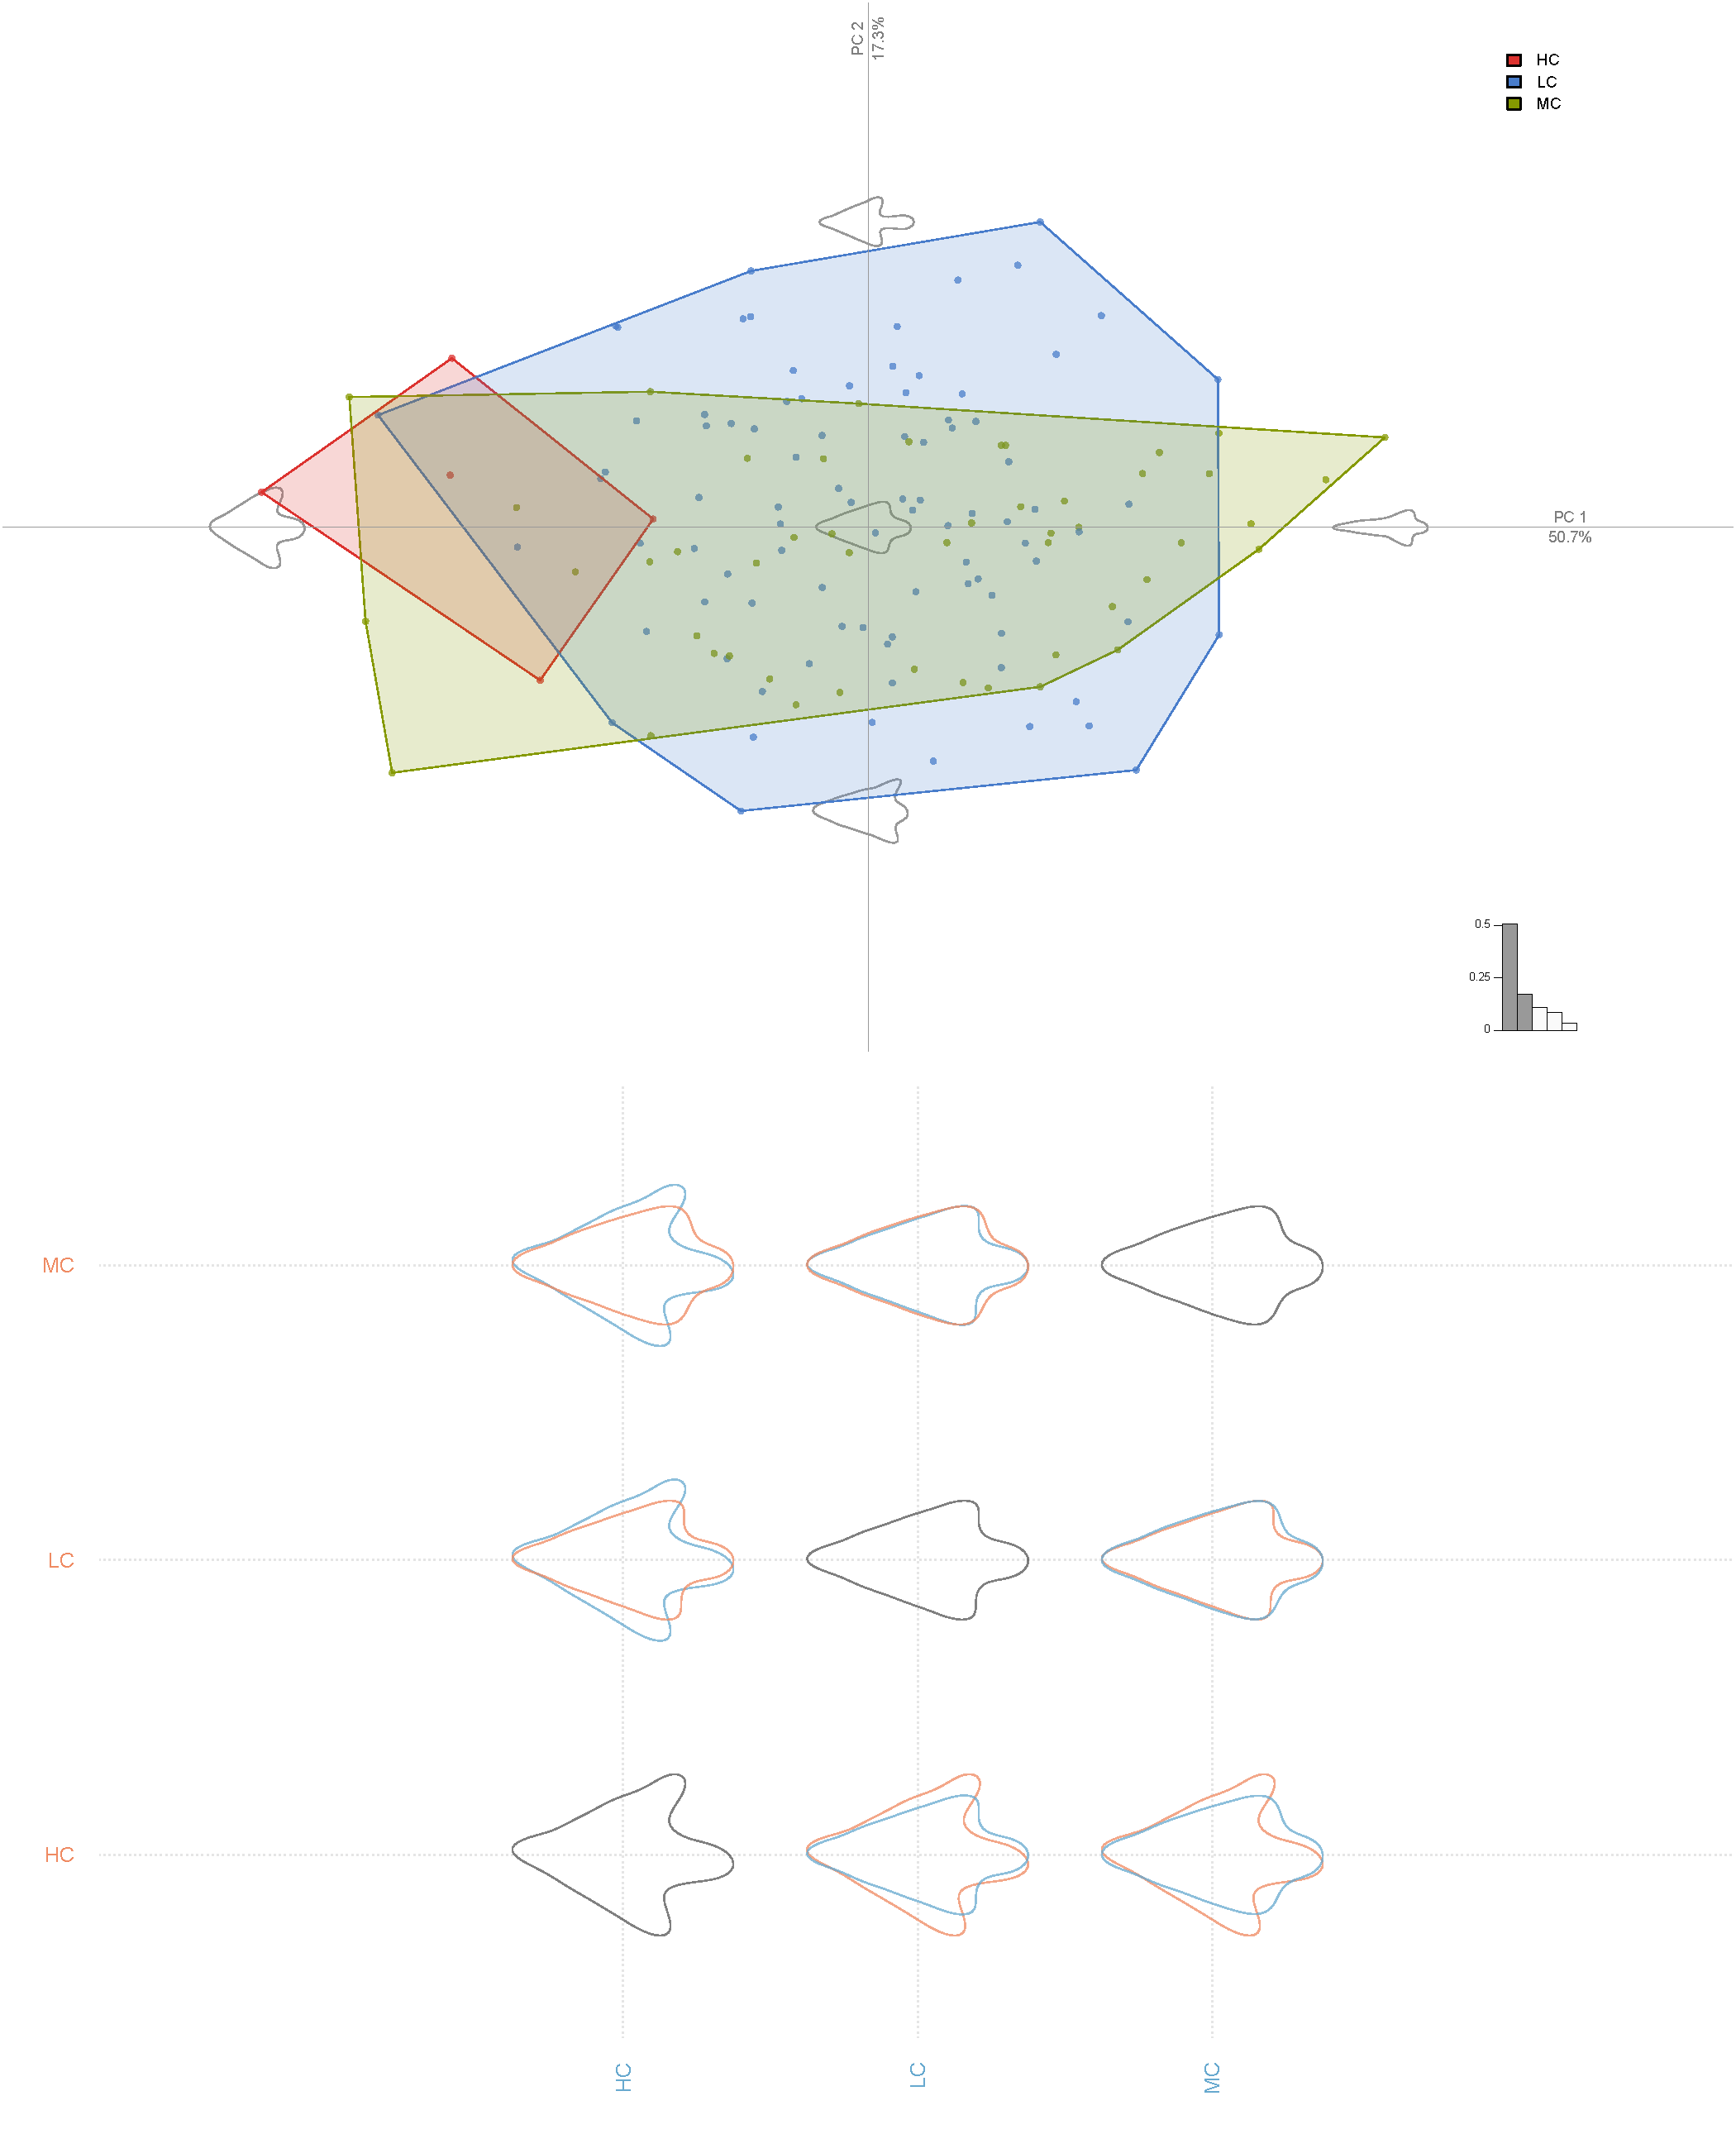
\includegraphics[width=0.9\linewidth]{temporal.pdf}
\caption{Principal components analysis plot (PC1/PC2) for Perdiz arrow points by temporal assignment (top), where green represents projectiles from the Middle Caddo period (CE 1250 - 1450), blue represents projectiles from the Late Caddo period (CE 1450 - 1680), and red represents projectiles from the Historic Caddo period (CE 1680+), as well as comparisons of mean shapes from each period (bottom) where MC, Middle Caddo; LC, Late Caddo; and HC, Historic Caddo. Additional information related to this figure, including the full results and code needed to reproduce it, can be found in the supplemental materials at \href{https://aksel-blaise.github.io/perdiz/elliptical-fourier-analysis.html}{https://aksel-blaise.github.io/perdiz/elliptical-fourier-analysis.html} and \citealp{RN8980}.}
\label{fig:gmtemp}
\end{figure}

\begin{table}[tbh]\centering
\footnotesize
\caption{Pairwise MANOVA for temporal periods.}
\centering
\begin{tabular}{lccc}
\hline
 & Historic & Late & Middle\\
\hline
Historic & & \textbf{9.561e-07} & \textbf{6.203e-12}\\
Late & & & \textbf{5.950e-10}\\
\hline
\end{tabular}\\
\textit{All results significant.}
\label{tab:tab.shape.time}
\end{table}

The marked shift in Perdiz morphology in the Historic Caddo period articulates with the fluorescence of the fur trade, potentially indicating a shape change to a more lethal variant of the Perdiz arrow point. The long narrow stem and tip, acutely pointed and flaring barbs, and overly thin nature of Perdiz arrow points in the Historic Caddo period could represent design choices intentionally used to manufacture a projectile point with greater lethal efficiency. The tensile strength of such narrow stems and barbs would appear to be intentional functional deficits, particularly if these implements were employed as hafted cutting tools or for other similar functions. However, when the design is considered from a perspective of lethality, it makes sense as these components may have been designed to fail catastrophically, thus increasing bleeding or organ damage. A functional relationship between arrow point design and fracture/fragmentation patterns has been suggested by \citet{RN9008} in his study of Perdiz points from the Clemente and Herminia Hinojosa site (41JW8), which was also suggested by \citet{RN9009} for site 41LK67. Similar fragmentation patterns were documented by \citet{RN8999} for Perdiz points from the Jayroe site (41HM51).

The junctions of the stem/body and barbs/body represent likely points of failure that---upon impact---would shatter a complete point into several fragments; each with very sharp edges that would further increase haemorrhaging during wound creation. Thus, Perdiz arrow points would have functioned in modes similar to composite geometric microlith arrow points or the transverse arrowheads characteristic of Neolithic and later weapons of Europe and the greater Middle East. At present, there has been no analysis of Perdiz arrow point design that has considered this aspect of morphology and technological choice. To address these possibilities would require replication and firing experiments using Perdiz arrow points against targets to study breakage patterns, which would aid in expanding studies of fracture types and breakage patterns in archaeological examples.

To meet the demands of the hide trade, the Plains hunter killed an average of 44 buffalo per year; far beyond the typical average of six buffalo needed annually for subsistence \citep{RN39}. Thus, the later shift in Perdiz arrow point morphology may have articulated with a considerable economic need for improved lethal efficiency. By the 1680s, the Caddo fur/hide trade with Europeans was robust, and included bear, beaver, deer, otter, rabbit, raccoon, and others \citep{RN9005,RN39,RN8076}. When those resources were scarce, Caddo hunters worked in organised groups that would travel a minimum of four days to find buffalo on the plains and prairies \citep{RN9005,RN38}. When trading with the French in Natchitoches, bear's fat would fetch the highest price at 25 livres each, followed by buffalo hides (10 livres/each), and deerskins (35 sous/each) \citep{RN9005}.

\subsubsection*{Shape as a function of raw material}

Results of the multivariate analysis of variance (MANOVA) through a Hotelling-Lawley of 99 percent cumulative shape variance indicated a significant difference in Perdiz arrow point shape by raw material (\textit{Hotelling-Lawley}: 0.77286, \textit{F}: 2.5977, \textit{PR(>F)}: 9.226e-06) (Figure ~\ref{fig:gmrawmat}, top,  supplemental materials, and \citealp[Chapter 4]{RN8980}). A subsequent MANOVA with pairwise comparison demonstrated a significant difference in mean Perdiz arrow point shape for each raw material (Table ~\ref{tab:tab.shape.raw}, supplemental materials, and \citealp[Chapter 4]{RN8980}). Mean shapes plotted by raw material type (chert, quartzite, and silicified wood) indicate a difference in Perdiz arrow point stem length and bilateral asymmetry, where chert points appear more symmetrical with a longer stem (Figure ~\ref{fig:gmrawmat}, bottom). Perdiz arrow points manufactured using quartzite are the least symmetrical with the shortest stem; however, Perdiz arrow points manufactured using silicified wood are also asymmetrical, but with a longer stem.

\begin{figure}[!]\centering
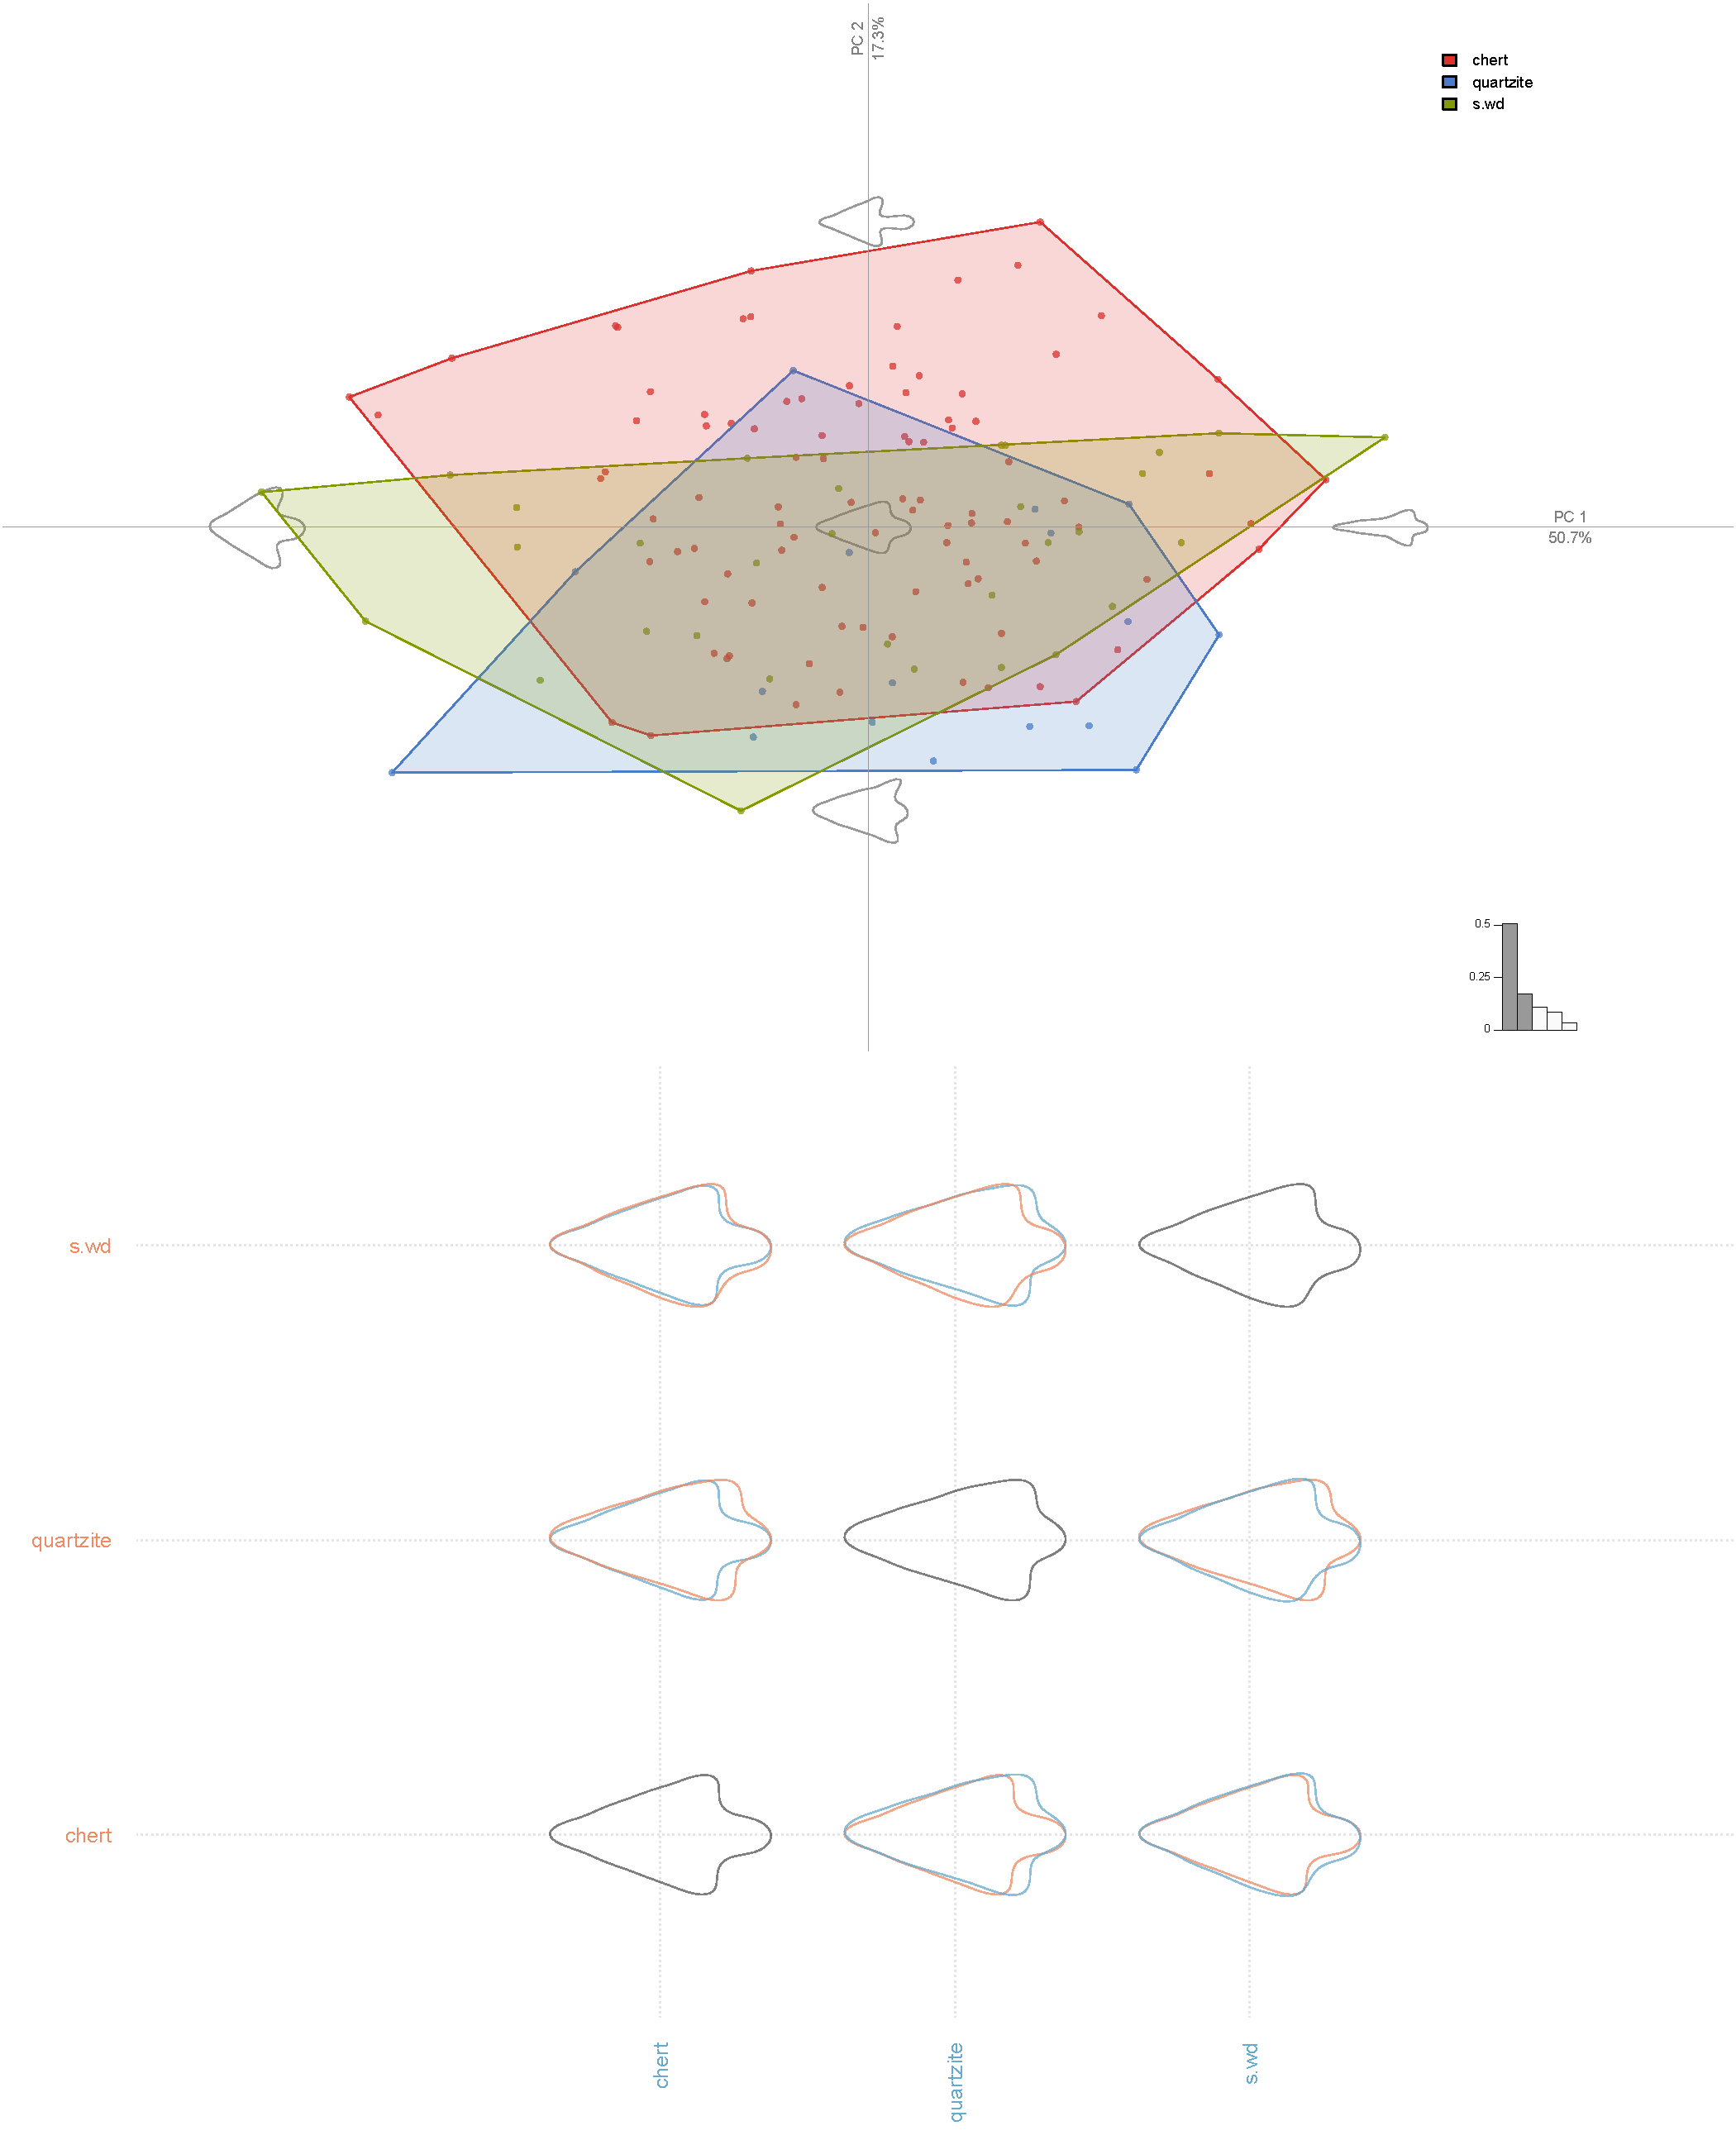
\includegraphics[width=\linewidth]{rawmat.pdf}
\caption{Principal components analysis plot (PC1/PC2) for Perdiz arrow points by raw material (top), where green represents silicified wood, blue represents quartzite, and red represents chert, as well as comparisons of mean shapes from each period (bottom). Additional information related to this figure, including the full results and code needed to reproduce it, can be found in the supplemental materials at \href{https://aksel-blaise.github.io/perdiz/elliptical-fourier-analysis.html}{https://aksel-blaise.github.io/perdiz/elliptical-fourier-analysis.html} and \citealp{RN8980}.}
\label{fig:gmrawmat}
\end{figure}

\begin{table}[tbh]\centering
\footnotesize
\caption{Pairwise MANOVA for raw materials.}
\centering
\begin{tabular}{lccc}
\hline
 & Chert & Quartzite & Silicified Wood\\
\hline
Chert & & \textbf{0.0050567} & \textbf{0.0007521}\\
Quartzite & & & \textbf{0.0228460}\\
\hline
\end{tabular}\\
\textit{All results significant.}
\label{tab:tab.shape.raw}
\end{table}

The documented morphological differences between Perdiz arrow points manufactured using different raw materials can be, at least in part, attributed to the varied geography associated with raw materials (see Figure ~\ref{fig:raw.map}). In the Caddo region, chert, quartzite, and silicified wood all occur as small (less than fist size) cobbles or nodules, often less than 10 cm in maximum dimension. This mode of raw material occurrence necessitated certain technological innovations to core reduction that allowed knappers to exploit small cobble material. Paramount among these was bipolar percussion and the use of punches and indirect percussion techniques \citep{RN8995,RN8996,RN8997,RN8998,RN2145}. These technological options to reduce small cores, produce flake blanks, and shape small hafted bifaces undoubtedly imposed technological and design constraints on Perdiz arrow point manufacture at the local and regional levels that were not factors in the \textit{classic} Toyah area where raw materials of sufficient size and quality are ubiquitous. 

While beyond the scope of this paper, it may be possible to accommodate such design constraints in later studies. The manufacturing trajectory of Perdiz arrow points from the southern Caddo area has not been the focus of technological lithic studies to date, unlike several central Texas studies that have addressed unique aspects of Perdiz point manufacture choices and their \textit{signatures} in the archaeological record \citep{RN8999,RN9000}. Raw material mode of occurrence is an influencing factor on the ultimate morphology and design of tools and is acknowledged as one that is difficult to control for in the analyses, since so little is known of Caddo Perdiz point manufacturing schemes.

\subsubsection*{Shape as a function of burial context}

Results of the multivariate analysis of variance (MANOVA) through a Hotelling-Lawley of 99 percent cumulative shape variance indicated a significant difference in Perdiz arrow point shape by burial context (\textit{Hotelling-Lawley}: 0.6106, \textit{F}: 4.1724, \textit{PR(>F)}: 8.86e-07) (Figure ~\ref{fig:gmcontext}, top and supplemental materials) \citep[Chapter 4]{RN8980}. Mean shapes plotted by burial context (recovered in/out) indicate a general difference in their overall plan view, where those from burial contexts exhibit a narrower blade, well established shoulders, and a stem that is both narrower and longer than those recovered outside of burial contexts (Figure ~\ref{fig:gmcontext}, bottom).

\begin{figure}[!]\centering
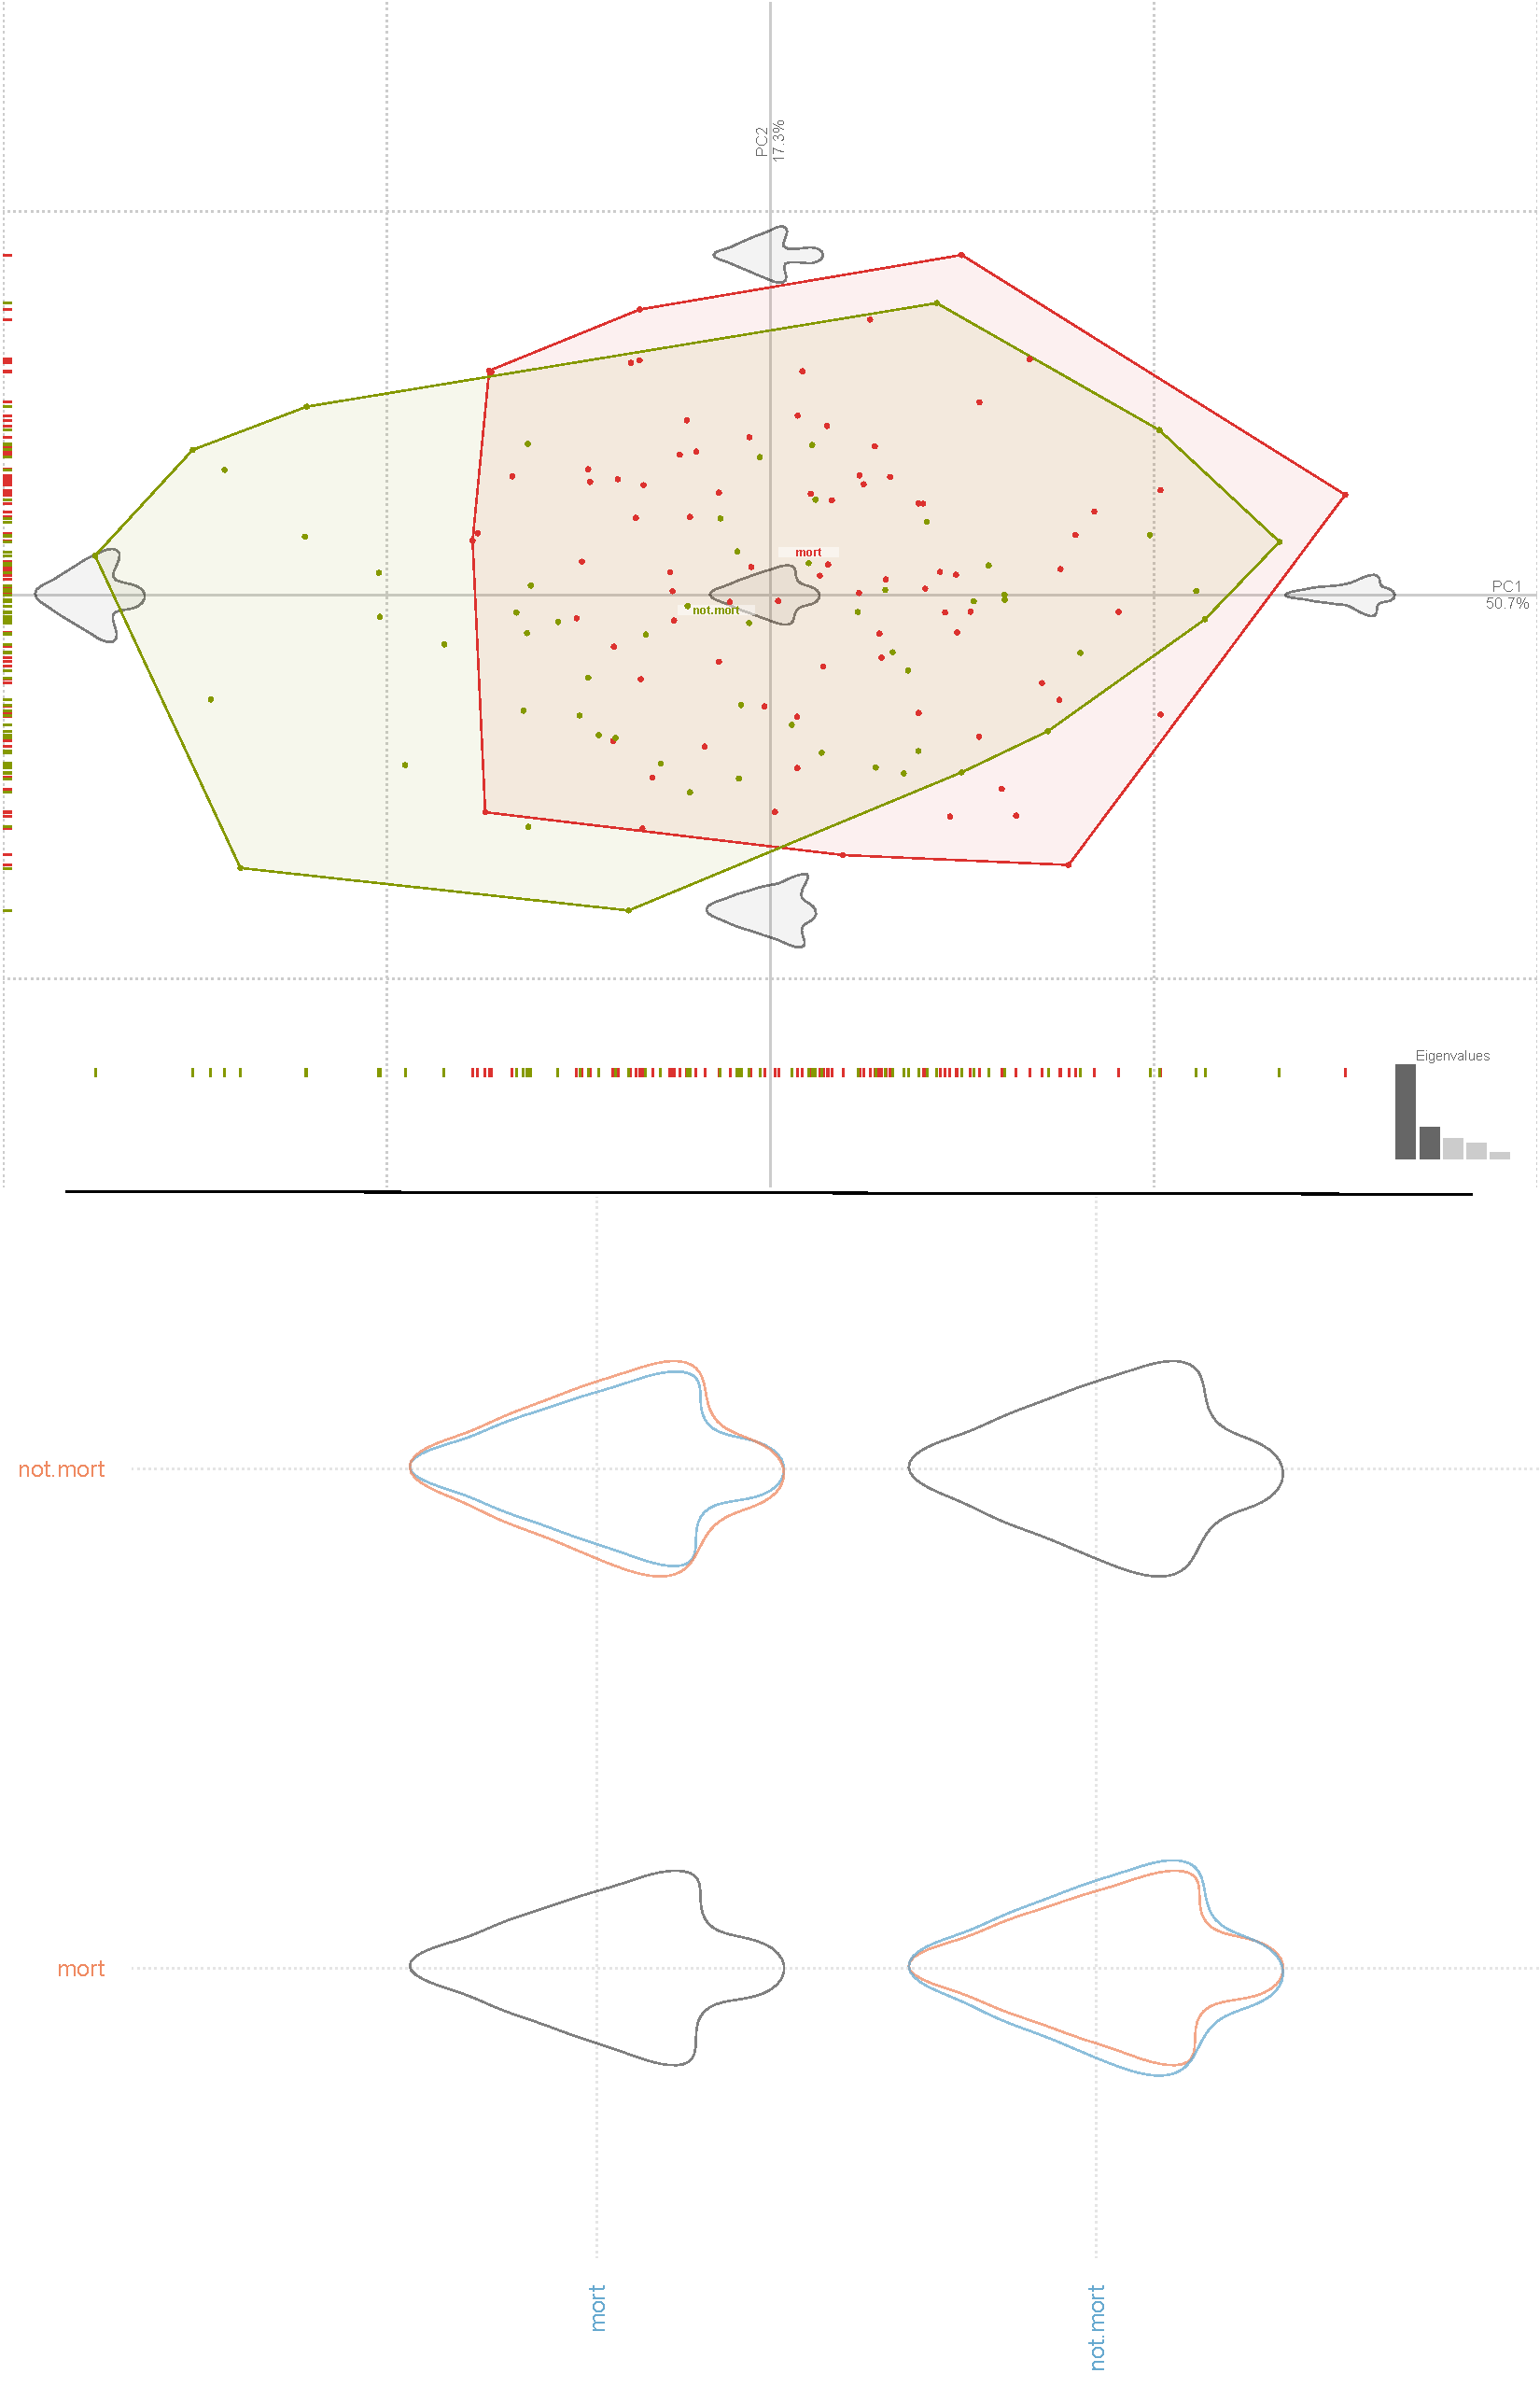
\includegraphics[width=\linewidth]{context.pdf}
\caption{Principal components analysis plot (PC1/PC2) for Perdiz arrow points by mortuary context (in/out) (top), where green represents projectiles \textit{not from} mortuary contexts, and red represents projectiles \textit{from} mortuary contexts, as well as comparisons of mean shapes from each context (bottom). Additional information related to this figure, including the full results and code needed to reproduce it, can be found in the supplemental materials at \href{https://aksel-blaise.github.io/perdiz/elliptical-fourier-analysis.html}{https://aksel-blaise.github.io/perdiz/elliptical-fourier-analysis.html} and \citealp{RN8980}.}
\label{fig:gmcontext}
\end{figure}

While this study has documented morphological differences among Perdiz arrow points from mortuary and non-mortuary contexts in the southern Caddo area, comparisons with non-mortuary point assemblages from the \textit{classic} Toyah area have not yet been pursued. Further comparisons of the Caddo and \textit{classic} Toyah area assemblages based on raw material differences would also be enlightening. If Perdiz arrow points from mortuary contexts were predominantly manufactured using chert sources from outside the Caddo area, then these could be inferred as grave offerings of non-Caddo visitors to the southern Caddo area as part of the symbolic maintenance of interaction spheres. Alternatively, it could reflect the import of non-local material by/for Caddo knappers to create suitable items for inclusion in a local mortuary event.

\section*{Discussion}

Recent studies of Caddo bottle and biface morphology have revealed a previously unrecognised north-south shape boundary for both bottles and bifaces, as well as a shape difference between Gahagan bifaces found in the southern Caddo area and central Texas \citep{RN8074,RN7927,RN8158,RN8370,RN8322,RN8312}. This exploratory effort expands upon that research programme to include arrow points as a means of analysing shape variability for a third artefact class of Caddo material culture. The analysis aggregated and analysed the variability in Perdiz arrow point shapes, and resulted in the identification of significant shape differences between temporal components, raw materials, and burial contexts. The analysis confirms that Perdiz arrow point morphology is labile, and that while some of the diagnostic shape differences are distinct, others are more nuanced.

A recent exploratory network analysis used the Historic Caddo ceramic and lithic types recovered from northeast Texas sites---which included Perdiz arrow points---led to the identification of a distinct, and previously unrecognised geographic shape difference (north-south) that occurs between the Neches and Sabine River basins in northeast Texas (Figure ~\ref{fig:fig.net}) \citep{RN8031}. Results indicated two larger Caddo communities of practice (Figure ~\ref{fig:fig.net}) \citep[Figure 16.4]{RN8031}, within which additional subcommunities of practice were hypothesised to be nested based upon the presence of common suites of material culture types \citep[Figures 16.5 and 16.6]{RN8031}. Some of the subcommunities articulate with known Caddo groups, while others do not; however, the networks serve as the requisite foundation for the production of reliable knowledge. Forthcoming morphological analyses will focus upon testing some of those hypotheses; however, additional Perdiz arrow points from within the Historic Caddo communities and subcommunities of practice must be integrated into subsequent studies if those analyses are to be pursued. The development of similar networks for the Middle and Late Caddo periods would have utility for constructing hierarchically-nested hypotheses related to the various ways in which the material culture of Caddo communities and subcommunities may have changed through time.

\begin{figure}[h!]\centering
\includegraphics[width=\linewidth]{fig.net.pdf}
\caption{Historic Caddo network generated using ceramic and lithic types, which include Perdiz arrow points (\href{https://osf.io/wd2zt/}{DOI 10.17605/OSF.IO/WD2ZT} and \citealt{RN8031}), illustrating two larger north (blue) and south (red) Caddo communities of practice. The communities were identified using a modularity statistic that identifies nodes that are more densely connected to one another than to the rest of the network \citep{RN8051,RN8024}.}
\label{fig:fig.net}
\end{figure}

Temporal differences identified in this study may provide the evidence needed to begin working through ontogenetic explanations that reflect Caddo approaches to the production, maintenance, and discard of Perdiz arrow points (sensu \citealt{RN5871}). There are differences in the approaches that Caddo knappers used to resolve design-based differences, which are represented at multiple levels: time, raw material, and burial context. As this research programme evolves, it will shift to a landmark-based approach, providing access to more advanced analytical methods, including phenotypic trajectory analysis \citep{RN8352,RN8561,RN8544,RN8560}, which could be used to investigate potential differential trajectories of phenotypic change through time, and by raw material, burial context, or community of practice. The results of the shape analysis by temporal period are the most pronounced; however, further research is warranted to assess whether morphological differences existed between the Caddo communities of practice identified in the Historic Caddo network analysis \citep{RN8031}.

Those temporal differences noted among Perdiz point assemblages in the Caddo region may indirectly document the adoption and regional refinement of the point type itself. It is not known whether Perdiz arrow points recovered from central Texas sites reflect similar intraspecific morphological transitions. If such differences do exist, it likely would not be for the same reasons noted in the Caddo area. Additional studies would be required to test this hypothesis.
Teasing these apart and assessing the overall influence of each would require directed technological and morphological studies that are beyond the scope of this study. Temporal changes in the type may provide indirect evidence associated with the initiation of extra-regional interaction with Toyah groups beyond the Caddo area. There is evidence of such interactions based on the presence of Caddo ceramics from Toyah sites scattered across central Texas \citep{RN9001}. \citet{RN6910} discussed the concept of a southern Plains macroeconomy with cores or nodes consisting of Pueblo and Caddo villages or areas. \citet{RN6046} and \citet{RN6910} both noted the importance of bison hides and bison products in exchange between the southern Plains and Caddo heartlands. \citet{RN6910} speculated that the Caddo region may be of greater importance than the Pueblo region with regard to trade with Plains groups, noting that Caddo artefacts (mainly pottery) are more common than items from the Southwest, which is true for the Toyah area as well \citep{RN8999}.

Perdiz arrow point shapes associated with raw materials used by Caddo knappers to manufacture Perdiz arrow points (chert, quartzite, and silicified wood) were found to differ significantly (Table ~\ref{tab:tab.shape.raw}, Figure ~\ref{fig:gmrawmat}, and supplementary materials \citealp{RN8980}). Unlike ceramic vessels, projectile points represent a single component of a larger technological system (assumed to be the bow and arrow) that archaeologists have been privy to in only the rarest of cases, due primarily to issues of preservation. The degree to which Perdiz arrow points were commodities enlisted for trade and exchange is not understood, and tools like the raw material retouch index posited by \citet{RN6541} may hold additional value for assessing relative raw material desirability in and among Caddo assemblages. \citet{RN6363} posited that design is an integral component of mobile toolkits, as a means of mitigating risks associated with raw material scarcity, but noted limits related to transporting technological material. Thus, the ideal design is one which provides the greatest potential utility relative to the cost of transport \citep{RN6363}. Whether design-based differences associated with raw material choice articulated with Caddo cultural or technological differences remains unknown.

It may be that differences in shape based upon raw material choices were related to both Caddo cultural and technological preferences. Certainly, the predominance of chert points incorporated into mortuary contexts by the Late Caddo period is a significant aspect of mortuary behaviour not seen prior to that time. While all raw materials behave similarly in procuring bison or other game, the almost exclusive use of chert in mortuary contexts may be representative of what was considered an appropriate \textit{offering} during the mortuary event; and may have been related to strengthening extra-regional relationships with other groups. Cherts in general, or cherts from particular source areas, may have been considered more appropriate for the manufacture of Perdiz points that were to be included in mortuary contexts.  

That Perdiz points come to figure prominently in the Caddo region by the Late Caddo period suggests that they represent an adopted piece of technology from beyond the Caddo region—given what is presently known of the distribution of Perdiz technology from the \textit{classic} Toyah region of central Texas. The point style may represent Caddo participation in extra regional social and/or economic networks oriented toward bison procurement and perhaps hide exchange \citep{RN9002}. Morphological differences between Caddo region Perdiz points from mortuary and non-mortuary contexts may express functional choices or design limitations between points manufactured using different materials. If significant design differences exist between Perdiz arrow points from Caddo contexts and areas outside the Caddo region, central Texas for instance, one could speculate that functional design-based differences may occur within the type. Perhaps one design achieved greater utility in heavily forested regions, and the other in regions that included more open oak and savannah grasslands.

Differences in burial contexts may reflect socially-distinct forms; some utilitarian, and others symbolic \citep[69]{RN8989}. However, utilitarian and symbolic characteristics associated with Perdiz arrow points in the southern Caddo area remain unknown. This analysis demonstrated a significant shape difference in Perdiz arrow points recovered from mortuary and non-mortuary contexts (Figure ~\ref{fig:gmcontext} and \citealt{RN8980}) in which those Perdiz arrow points from outside of mortuary contexts generally express a more oblique shoulder angle, and a broader blade than those recovered from mortuary contexts. As mentioned above, Perdiz arrow points are considered to be one component of a reliable tool \citep{RN5873}, which nests within the larger category of curated tools \citep{RN5880}. It is possible that the Perdiz arrow points recovered from mortuary contexts articulate with a more symbolic shape, and those recovered outside of mortuary contexts with utilitarian use, possibly due to a manufacturing process that was more expedient or time constrained. Thus, the shape of Perdiz arrow points recovered from burials may convey morphological traits that align more closely with locally-diagnostic variants expressive of differential \textit{design intent}.

While beyond the purview of this study, the function of Perdiz arrow points---whether utilised as part of a larger projectile-based system or for sawing, cutting, or piercing---may become evident through observing the location and type of retouch or use-wear, providing those data necessary to address potential conceptual shifts in archaeological interpretations \citep{RN8990,RN8991,RN8992,RN6342}. \citet{RN8994} and \citet{RN8993} posited range, accuracy, killing power, and stability to be four major constraints of a functioning missile; each of which could be impacted through retouch. Studies of Perdiz use-wear and retouch present a unique challenge, since many of the arrow points used in this study have been---or are scheduled to be---repatriated, and determinations would have to be conducted through an analysis of previously-collected images.

\section*{Conclusion}

This study has documented significant differences in Perdiz arrow point shape across the Middle, Late, and Historic Caddo periods. Quantifiable changes have been documented in arrow point shoulder angles across Caddo history ranging from obtuse in the Middle Caddo period to acute by the Historic Caddo period. The dramatic shift in Perdiz arrow point morphology in the Historic Caddo period correlates temporally with the fluorescence of the fur or peltry trade. It is speculated that at least some of the morphological or template-based design changes may relate to Caddo efforts to increase the lethality of the weapon. Perdiz arrow point shape was also shown to differ by raw material type. The general trend involved both arrow point stem length and bilateral asymmetry. Chert points were found to be more symmetrical with longer stems, while quartzite specimens were the least symmetrical with the shortest stems, and silicified wood points expressed attributes similar to quartzite, but with longer stems. Some of this variance can be explained by the geographic occurrence of raw materials. In particular, the mode of occurrence (gravels) for raw materials in northeast Texas and the Caddo region, versus the bedded and large cobble occurrence of cherts in the \textit{classic} Toyah region of Central Texas. Significant differences in Perdiz arrow point shape were also documented by mortuary contexts, where those recovered from burials generally exhibited narrower blades, well made shoulders/barbs, and more narrow, longer stems.

Results of an exploratory network analysis utilising Historic Caddo ceramic and lithic types from multiple northeast Texas sites (including Perdiz points) identified a north-south divide situated between the Neches and Sabine River drainages. This phenomenon is interpreted to represent two distinct Caddo communities of practice. Results of this study illustrate significant differences in those approaches that Caddo flintknappers used to resolve design constraints and weapon-based \textit{design intent}. These choices are reflected across time, raw material, and burial context (mortuary/non-mortuary). Future detailed studies of these issues may provide additional information relevant to regional refinements of the Perdiz type. Many of these findings are directly applicable to the continued development of testable hypotheses regarding regional and locally-based differences regarding how Perdiz arrow points were conceived of, and designed, in and among various communities of practice. Such hypotheses can be enlightening with regard to how artisans meaningfully integrated cultural and material constraints of formal artefact design.

\section*{Acknowledgments}

We express our gratitude to the Caddo Nation of Oklahoma and the Anthropology and Archaeology Laboratory at Stephen F. Austin State University for the requisite permissions and access to the NAGPRA items in the Turner collection. Thanks to Dan McGregor for information on Pisgah Ridge chert, and to Christian Hoggard, David K. Thulman, Michael J. O'Brien, and Julian A Sitters, as well as the editor and reviewers for their pre- and post-submission comments and constructive criticisms, which further improved the manuscript. Components of the analytical workflow were developed and funded by a Preservation Technology and Training grant (P14AP00138) to RZS from the National Center for Preservation Technology and Training, as well as grants to RZS from the Caddo Nation of Oklahoma, National Forests and Grasslands in Texas (15-PA-11081300-033) and the United States Forest Service (20-PA-11081300-074).

\section*{Data Management}

Data and analysis code associated with the geometric morphometric components of this study can be accessed through the supplementary materials (\href{https://aksel-blaise.github.io/perdiz/}{https://aksel-blaise.github.io/perdiz/}) or \href{https://github.com/aksel-blaise/perdiz}{GitHub repository}, which is digitally curated on the Open Science Framework \href{https://osf.io/dej74/}{DOI 10.17605/OSF.IO/DEJ74}, where additional data associated with the chi-square analysis are provided.

\bibliography{mybibfile}

\end{document}
